
\begin{figure}
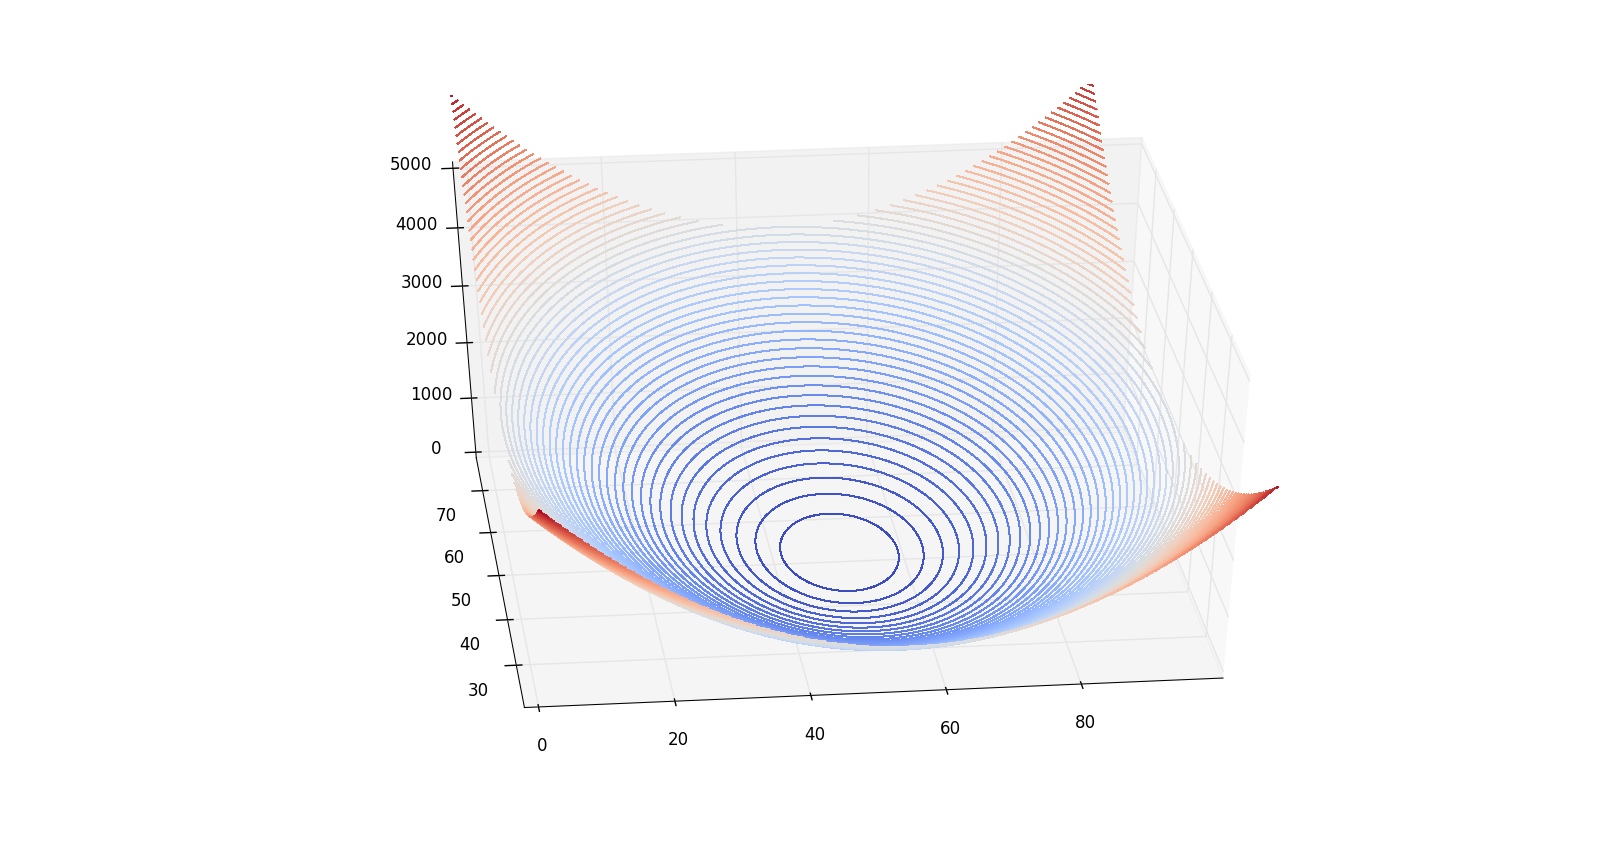
\includegraphics[height=.3\vsize]{fig/arriv1.png}
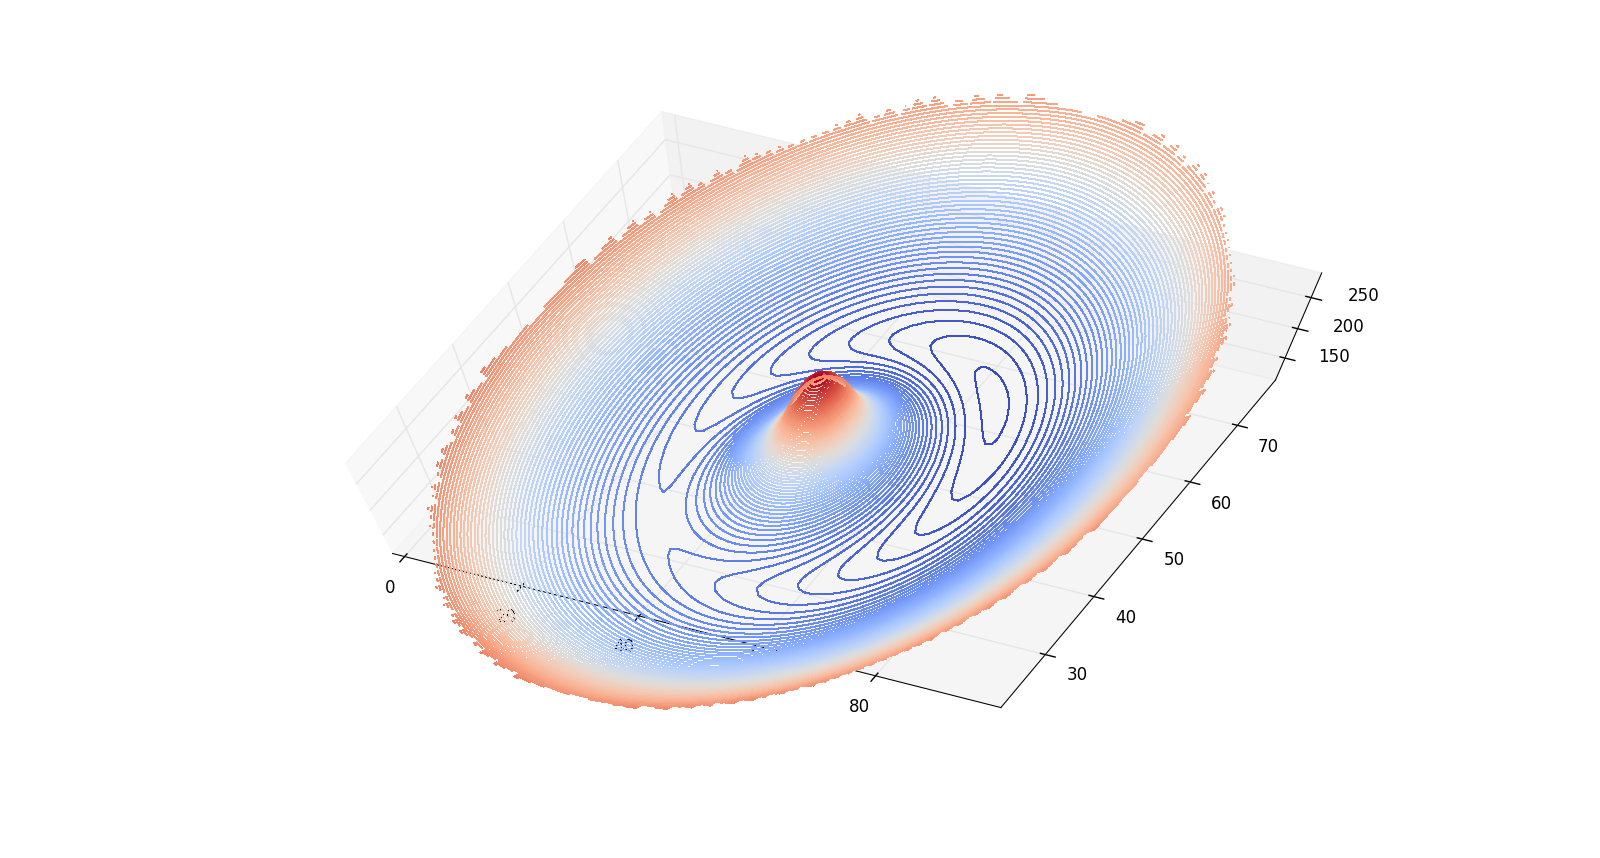
\includegraphics[height=.3\vsize]{fig/arriv2.png}
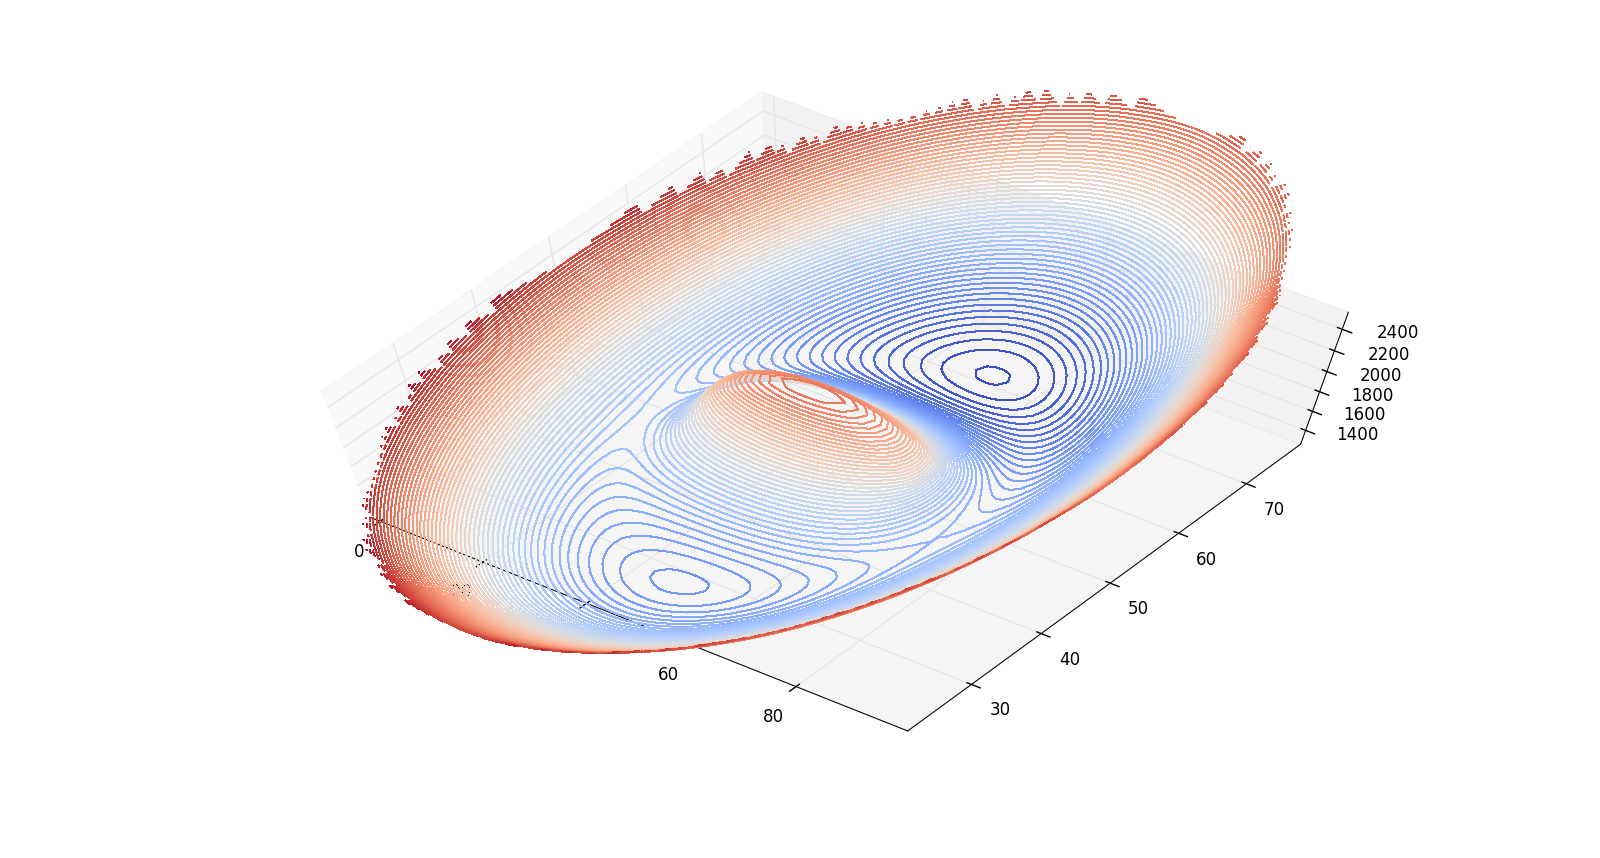
\includegraphics[height=.3\vsize]{fig/arriv3.png}
\caption{Arrival-time surfaces\label{fig:arriv}}
\end{figure}

\begin{figure}
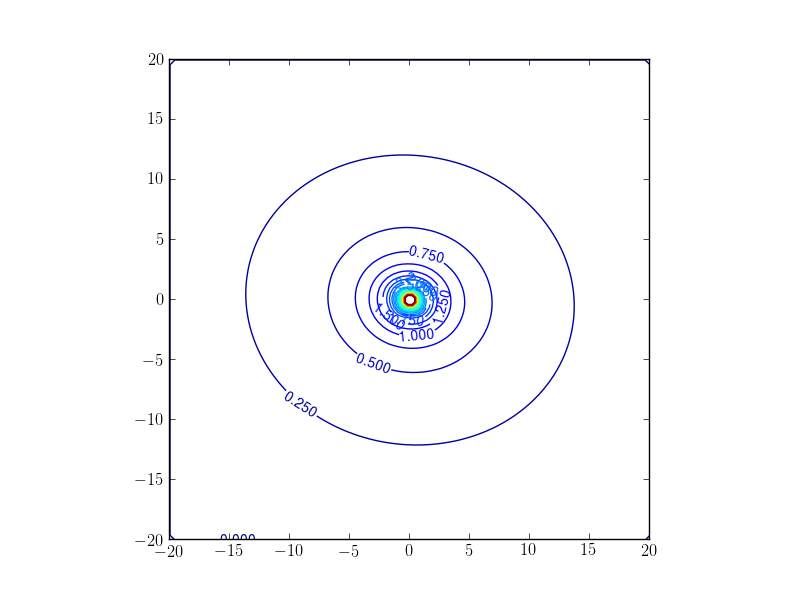
\includegraphics[width=.32\hsize]{fig/ASW0000ar2Q_kappa.png}
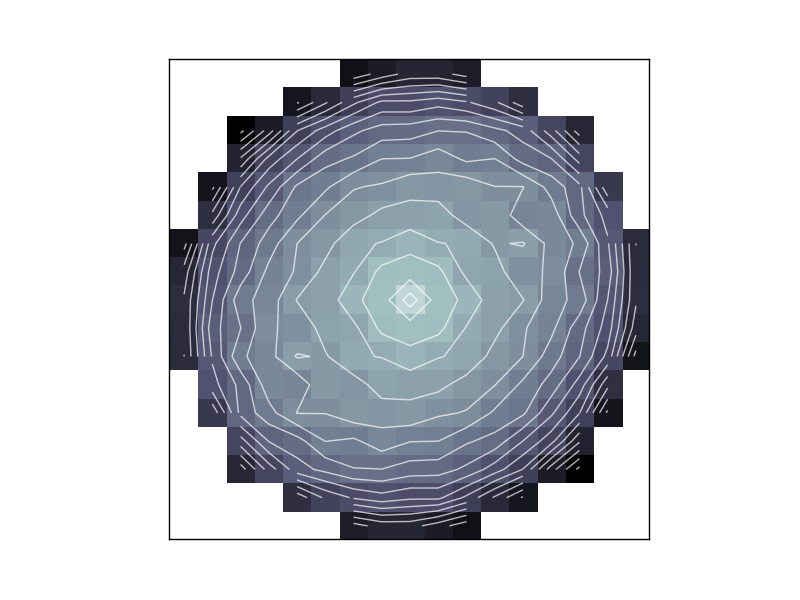
\includegraphics[width=.32\hsize]{fig/ASW0000ar2_kappa.png}
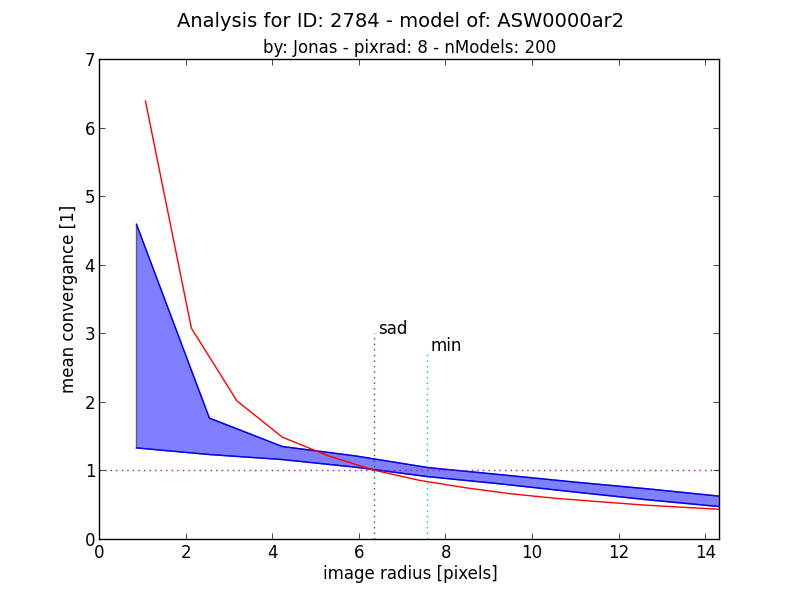
\includegraphics[width=.32\hsize]{fig/ASW0000ar2_menc.png} \\
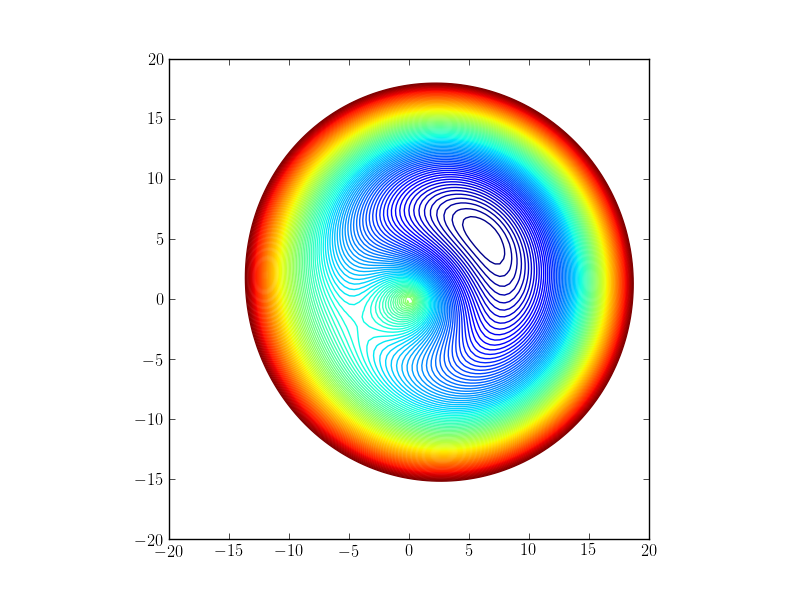
\includegraphics[width=.32\hsize]{fig/ASW0000ar2Q_arriv.png}
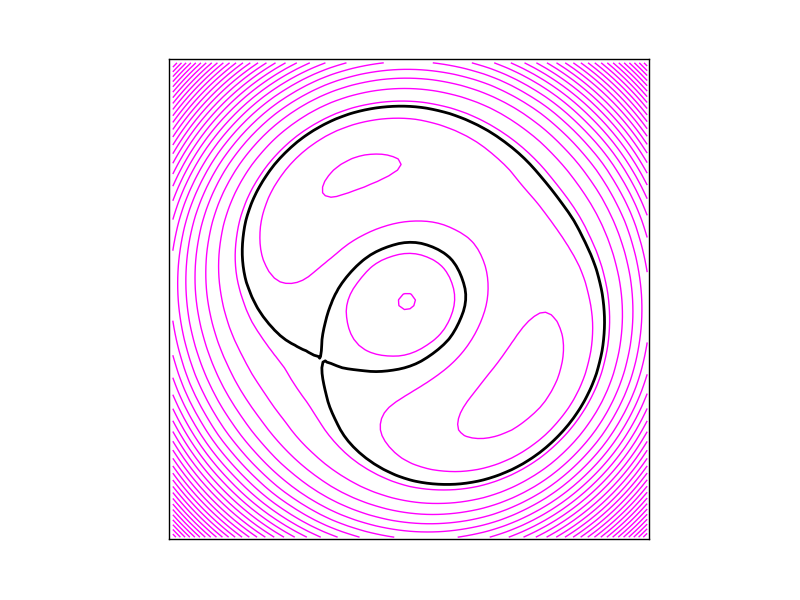
\includegraphics[width=.32\hsize]{fig/ASW0000ar2_arriv.png}
\caption{A simple two-image lensed quasar.  The minimum and saddle are
  identified correctly.  The mean model shows two spurious images, but
  the mean convergence in the region of images is good.
\label{fig:ASW0000ar2}}
\end{figure}